\documentclass[11pt]{beamer}

\usepackage[T1]{fontenc}
\usepackage[default]{opensans}
\usepackage{hyperref}
\usepackage{tikz}
\usepackage[dvipsnames]{xcolor}
\usepackage{graphicx}

\hypersetup{
  colorlinks=true,
  urlcolor=blue,
  linkcolor=blue,
  citecolor=blue
}

\usetheme{default}
\usecolortheme{dolphin}
\useinnertheme{circles}

\title{Rotaciones y ángulos de Euler en \(\mathbb{R}^3\)}
\subtitle{Álgebra lineal · Introducción a sistemas dinámicos y a la orientación y navegación}
\author[M. Osipova]{Mariia Osipova\\[3pt]\textit{mosipova@udesa.edu.ar}}
\institute{\\[12pt]Bajo la supervisión de Juan Felipe Perdomo}
\date[12 dic 2025]{12 de diciembre 2025}

%----------------------------------------------------------------------------------------
%fuentes
%----------------------------------------------------------------------------------------
\newcommand{\srcBarfoot}{\href{https://asrl.utias.utoronto.ca/~tdb/bib/barfoot_ser17.pdf}{Barfoot (2017)}}
\newcommand{\srcShuster}{\href{https://ru.scribd.com/doc/155830038/A-Survey-of-Attitude-Representations}{Shuster (1993)}}
\newcommand{\srcSola}{\href{https://www.iri.upc.edu/people/jsola/JoanSola/objectes/notes/kinematics.pdf}{Sol\`a (2017)}}
\newcommand{\srcMarkley}{\href{https://notes.jaydickson.net/assets/resources/Textbooks/Markley\%20and\%20Crassidis\%20-\%202014\%20-\%20Fundamentals\%20of\%20Spacecraft\%20Attitude\%20Determination\%20.pdf}{Markley \& Crassidis (2014)}{Markley \& Crassidis (2014)}}

\newcommand{\SourceLine}[1]{\vfill{\tiny\textcolor{gray}{Fuentes: #1}}}

%----------------------------------------------------------------------------------------

%----------------------------------------------------------------------------------------

\begin{document}

%----------------------------------------------------------------------------------------
%	TITLE SLIDE
%----------------------------------------------------------------------------------------

\begin{frame}
	\titlepage % Output the title slide, automatically created using the text entered in the PRESENTATION INFORMATION block above
\end{frame}

%----------------------------------------------------------------------------------------
%	TABLE OF CONTENTS SLIDE
%----------------------------------------------------------------------------------------

% The table of contents outputs the sections and subsections that appear in your presentation, specified with the standard \section and \subsection commands. You may either display all sections and subsections on one slide with \tableofcontents, or display each section at a time on subsequent slides with \tableofcontents[pausesections]. The latter is useful if you want to step through each section and mention what you will discuss.

\begin{frame}{Resumen de la presentación}
  \tableofcontents
\end{frame}

%------------------------------------------------

\section{Introducción}

%------------------------------------------------

\begin{frame}
    \frametitle{Introducción}

%    \begin{columns}[T]
%        \begin{column}{0.5\textwidth}
%            En esta presentación estudiamos rotaciones en \(\mathbb{R}^3\) y distintas representaciones de la orientación (\emph{attitude}):
%            matrices de rotación, ángulos de Euler y cuaterniones.
%        \end{column}
%
%        \begin{column}{0.5\textwidth}
%            \begin{tikzpicture}[scale=2.3, line cap=round, line join=round]
%              % axes
%              \draw[->,thick] (-0.1,0) -- (1.4,0) node[right] {$x$};
%              \draw[->,thick] (0,-0.1) -- (0,1.2) node[above] {$y$};
%
%              % angle
%              \def\th{35}
%
%              % original vector (along x)
%              \draw[thick] (0,0) -- (1,0) node[midway,below] {$v$};
%
%              % rotated vector
%              \draw[thick] (0,0) -- ({cos(\th)},{sin(\th)}) node[above right] {$R(\theta)v$};
%
%              % arc for theta
%              \draw[thick] (0.35,0) arc (0:\th:0.35);
%              \node at ({0.45*cos(\th/2)},{0.45*sin(\th/2)}) {$\theta$};
%
%              % optional: point markers
%              \fill (1,0) circle (0.5pt);
%              \fill ({cos(\th)},{sin(\th)}) circle (0.5pt);
%            \end{tikzpicture}
%        \end{column}
%    \end{columns}

    En esta presentación estudiamos rotaciones en \(\mathbb{R}^3\) y distintas representaciones de la orientación (\emph{attitude}):
    matrices de rotación, ángulos de Euler y un poco de cuaterniones. \vspace{6pt}

\end{frame}

%------------------------------------------------

\begin{frame}
    \frametitle{Introducción}

    Los vehículos (por ejemplo, robots, satélites, aeronaves) suelen tener libertad para trasladarse y rotar. Matemáticamente, tienen seis grados de libertad: tres en traslación y tres en rotación. Esta configuración geométrica de seis grados de libertad se conoce como the pose (posición y orientación) del vehículo.

    \begin{figure}[htbp]
      \centering
      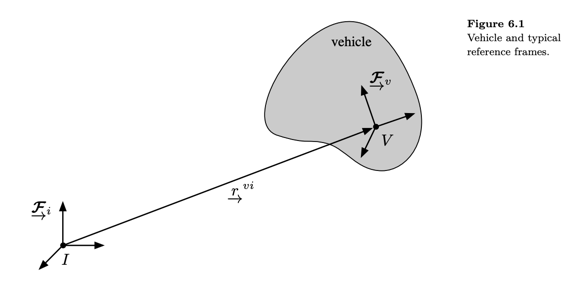
\includegraphics[width=0.7\textwidth]{imagenes/img}
      \label{fig:plot}
    \end{figure}

    \SourceLine{\srcBarfoot, p. 173.}
\end{frame}

%------------------------------------------------

\begin{frame}
\frametitle{Introducción}

    Definimos un sistema tridimensional con tres ejes ortogonales \((x,y,z)\) y los planos coordenados asociados.\\[8pt]

    \begin{columns}[T]
        \begin{column}{0.33\textwidth}
            \centering
            \begin{tikzpicture}[scale=1.6, line cap=round, line join=round]
              \draw[->,thick, red] (-0.1,0) -- (1.4,0) node[right] {$x$};
              \draw[->,thick, green!70!black] (0,-0.1) -- (0,1.2) node[above] {$y$};
            \end{tikzpicture}
        \end{column}

        \begin{column}{0.33\textwidth}
            \centering
            \begin{tikzpicture}[scale=1.6, line cap=round, line join=round]
              \draw[->,thick, red] (-0.1,0) -- (1.4,0) node[right] {$x$};
              \draw[->,thick, blue] (0,-0.1) -- (0,1.2) node[above] {$z$};
            \end{tikzpicture}
        \end{column}
        \begin{column}{0.33\textwidth}
            \centering
            \begin{tikzpicture}[scale=1.6, line cap=round, line join=round]
              \draw[->,thick, green!70!black] (-0.1,0) -- (1.4,0) node[right] {$y$};
              \draw[->,thick, blue] (0,-0.1) -- (0,1.2) node[above] {$z$};
            \end{tikzpicture}
        \end{column}
    \end{columns}

    \vfill
    {\footnotesize\textcolor{gray}{%
    Note: Podríamos partir de \((x_1,x_2,x_3)\), pero en muchos artículos y apuntes se usa \((x,y,z)\); por eso adopté esta notación.}}

\end{frame}

%------------------------------------------------

\begin{frame}
\frametitle{Introducción}

    \begin{columns}[T]
        \begin{column}{0.55\textwidth}
            A este sistema lo llamamos ``Body-Fixed Axes``: la orientación (\emph{attitude}) del objeto queda determinada por la orientación de estos ejes en el espacio.
            En otras palabras, se trata de un sistema de coordenadas, digamos, ligado al objeto (por ejemplo, un avión o un dron) que gira conjuntamente con él.
        \end{column}

        \begin{column}{0.45\textwidth}
            \begin{tikzpicture}[scale=2, line cap=round, line join=round]
              \draw[->,thick,green!70!black]   (0,0) -- (1.3,0) node[right] {$y$};
              \draw[->,thick,blue] (0,0) -- (0,1.2) node[above] {$z$};
              \draw[->,thick,red]  (0,0) -- (-0.7,-0.7) node[below left] {$x$};
            \end{tikzpicture}
        \end{column}
    \end{columns}

\end{frame}

%------------------------------------------------

\begin{frame}
\frametitle{Introducción}

    \begin{columns}[T]
        \begin{column}{0.55\textwidth}
            La posición de un punto en un vehículo se puede describir con un vector \(\vec{r}_{vi}\), que consiste de tres componentes.

            \[
            \vec{r}_{vi} =
            \begin{bmatrix}
            x \\
            y \\
            z
            \end{bmatrix}
            \] \vfill

            Consideraremos un vector como una cantidad \(\vec{r}_{vi}\) con longitud y dirección.

        \end{column}

        \begin{column}{0.45\textwidth}
            \begin{tikzpicture}[scale=2, line cap=round, line join=round]
              \draw[->,thick,green!70!black]   (0,0) -- (1.3,0) node[right] {$y$};
              \draw[->,thick,blue] (0,0) -- (0,1.2) node[above] {$z$};
              \draw[->,thick,red]  (0,0) -- (-0.7,-0.7) node[below left] {$x$};

              \draw[->,thick,black] (0,0) -- (0.9,0.8) node[above right] {$\vec{r}_{vi}$};

            \end{tikzpicture}
        \end{column}
    \end{columns}

    \vfill
    {\footnotesize\textcolor{gray}{%
    Note: \(v\) -- vehicle; \(i\) -- punto \(i\) en ese objeto.
    Entonces \(\vec{r}_{vi}\) es el vector desde el origen del sistema de coordenadas
    del vehículo hasta el punto \(i\).}}

\SourceLine{\srcBarfoot, p. 174.}

\end{frame}

%------------------------------------------------

\begin{frame}
\frametitle{Introducción}

    \begin{columns}[T]
        \begin{column}{0.55\textwidth}
            Ahora nos gustaría introducir una rotación alrededor de un eje.

            El movimiento de rotación se describe expresando la orientación de un sistema
            de referencia en el vehículo, \(F_v\), con respecto a otro sistema, \(F_i\).
            La Figura 6.1 muestra la configuración típica de un vehículo monocasco.

        \end{column}

        \begin{column}{0.45\textwidth}
            \begin{tikzpicture}[scale=2, line cap=round, line join=round]


             \draw[->,thick,green!70!black]   (0,0) -- (1.3,0) node[right] {$y$};
             \draw[->,thick,blue] (0,0) -- (0,1.2) node[above] {$z$};
             \draw[->,thick,red]  (0,0) -- (-0.7,-0.7) node[below left] {$x$};

%             \def\h{0.8}   % высота по x3
%             \def\a{0.20}  % большой радиус эллипса (ширина)
%             \def\b{0.08}  % малый радиус (перспектива)
%             \def\st{125}
%             \def\en{425}
%
%            \draw[CadetBlue, thick, ->]
%              (0,\h) ++({\a*cos(\st)},{\b*sin(\st)})
%              arc[start angle=\st, end angle=\en, x radius={\a}, y radius={\b}];
%
%            \node[CadetBlue] at (0.20,\h+0.25) {$\psi$};

             \draw[->,thick,black] (0,0) -- (0.9,0.8) node[above right] {$\vec{r}_{vi}$};

            \node[right] at (0.8,0.3) {$\vec{F}_1$};
            \end{tikzpicture}
        \end{column}
    \end{columns}

\end{frame}

%------------------------------------------------

\begin{frame}
\frametitle{Introducción}

    \begin{columns}[T]
        \begin{column}{0.55\textwidth}
            Ahora nos gustaría introducir una rotación alrededor de un eje.

            El movimiento de rotación se describe expresando la orientación de un sistema
            de referencia en el vehículo, \(F_v\), con respecto a otro sistema, \(F_i\).
            La Figura 6.1 muestra la configuración típica de un vehículo monocasco.

        \end{column}

        \begin{column}{0.45\textwidth}
            \begin{tikzpicture}[scale=2, line cap=round, line join=round]


             \draw[->,thick,green!70!black]   (0,0) -- (1.3,0) node[right] {$y$};
             \draw[->,thick,blue] (0,0) -- (0,1.2) node[above] {$z$};
             \draw[->,thick,red]  (0,0) -- (-0.7,-0.7) node[below left] {$x$};

             \def\h{0.8}   % высота по x3
             \def\a{0.20}  % большой радиус эллипса (ширина)
             \def\b{0.08}  % малый радиус (перспектива)
             \def\st{125}
             \def\en{425}

            \draw[CadetBlue, thick, ->]
              (0,\h) ++({\a*cos(\st)},{\b*sin(\st)})
              arc[start angle=\st, end angle=\en, x radius={\a}, y radius={\b}];

            \node[CadetBlue] at (0.20,\h+0.25) {$\psi$};

             \draw[->,thick,black] (0,0) -- (0.9,0.8) node[above right] {$\vec{r}_{vi}$};

            \node[right] at (0.8,0.3) {$\vec{F}_1$};
            \end{tikzpicture}
        \end{column}
    \end{columns}

\end{frame}

%------------------------------------------------

\section{Bibliografía}

%------------------------------------------------

\begin{frame}
\frametitle{Bibliografía}

\small
\begin{itemize}
  \item T. D. Barfoot, \emph{State Estimation for Robotics}, Cambridge University Press, 2017.
  \item M. D. Shuster, ``A Survey of Attitude Representations'', \emph{Journal of the Astronautical Sciences}, 1993.
  \item J. Solà, ``Quaternion Kinematics for the Error-State Kalman Filter'', 2017.
  \item F. L. Markley, J. L. Crassidis, \emph{Fundamentals of Spacecraft Attitude Determination and Control}, Springer, 2014.
\end{itemize}
\end{frame}

%https://www.youtube.com/watch?v=D1lnrQg5NAM&t=1283s

%------------------------------------------------

%----------------------------------------------------------------------------------------


\end{document}